\section{Analisi di classificazione}\label{sec:class}

\subsection{Un nuovo caso di studio}

Si vuole ora passare a un problema di tipo diverso da quello dichiarato in
sezione \ref{sec:intro-abstract}.

Se prima il problema era determinare la richiesta del servizio di \emph{Bike
sharing}, ora ci si concentra su una delle due variabili risposta che finora
sono state ignorate (cfr. sez. \ref{sec:lin-risp}).

In particolare, si vuole capire in quali condizioni gli utenti non registrati
utilizzano maggiormente il servizio. Nella figura seguente è mostrato un
boxplot che mostra l'utilizzo del servizio di \emph{Bike sharing} da parte di
utenti non registrati presente nei dati a nostra disposizione.

\begin{figure}[H]
  \centering
  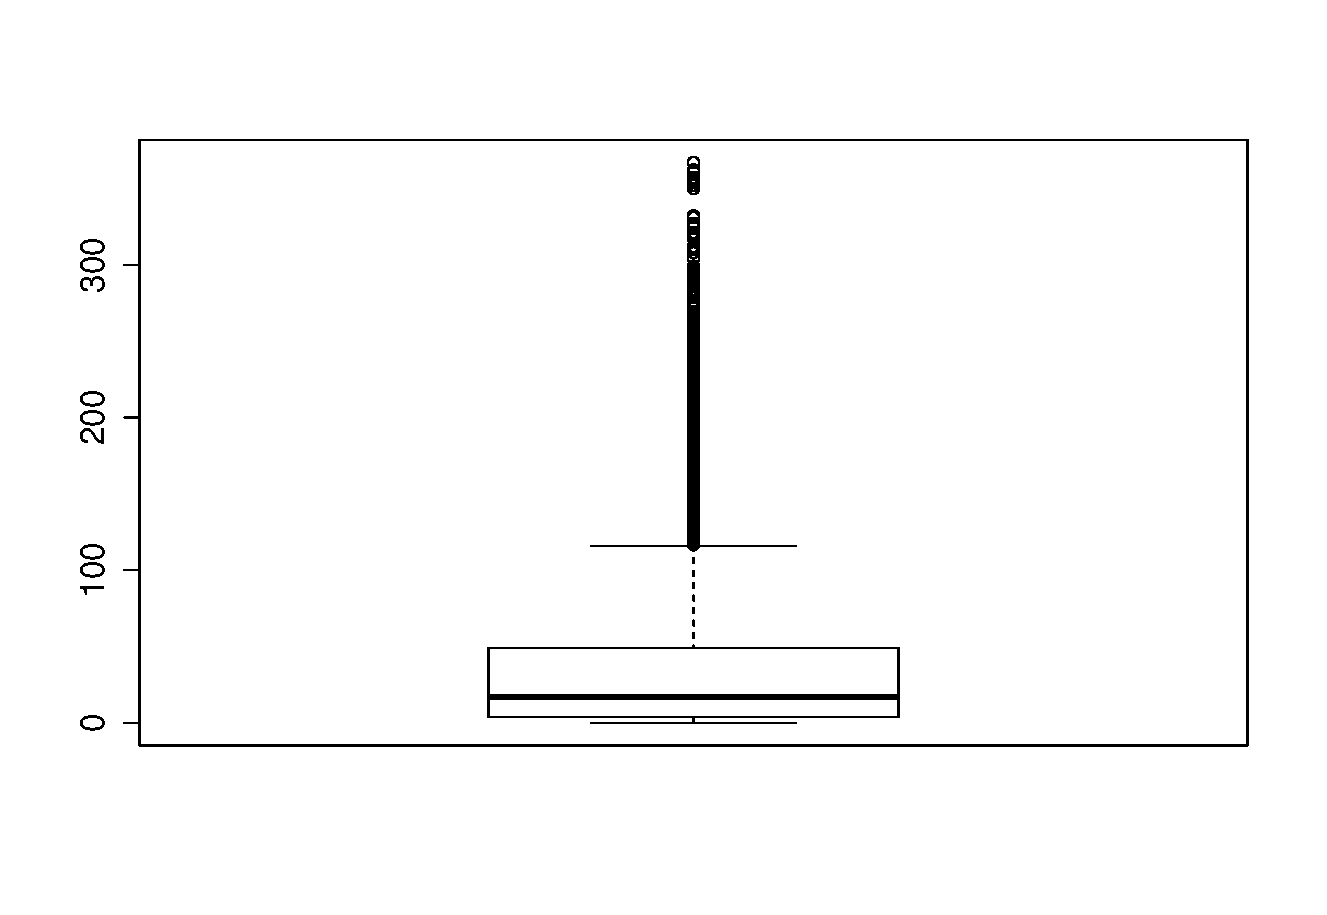
\includegraphics[width=.5\columnwidth]{images/class/boxplot-casual.eps}
  \caption{Boxplot per \texttt{train\$casual}}
  \label{fig:simplest-linear-model}
\end{figure}

Come si può vedere in figura, i dati sono molto concentrati verso valori bassi
di utilizzo (con mediana 18, trovata con il comando \texttt{summary} di R).
Guardando il boxplot, si sceglie 50 come soglia per distinguere se l'utilizzo
è elevato o meno\footnote{N.B. la soglia è puramente arbitraria}.

A questo punto si procede inserendo nel nostro workspace una variabile
``\texttt{aLotCasual}'' che avrà valori 1 o 0 a seconda che il servizio sia
stato utilizzato abbondantemente o meno da utenti non registrati (script
\ref{sec:script-populate-class}).

%%%%%%%%%%%%%%%%%%%%%%%%%%%%%%%%%%%%%%%%%%%%%%%%%%%%%%%%%%%%%%%%%%%%%%%%%%%%%%%
%%%%%%%%%%%%%%%%%%%%%%%%%%%%%%%%%%%%%%%%%%%%%%%%%%%%%%%%%%%%%%%%%%%%%%%%%%%%%%%

\subsection{Regressione lineare logistica}\label{sec:class-log-reg}

Come al solito, si parte sempre tentando di approssimare i nostri dati nel
modo più semplice possibile, ovvero con una retta.

In questo caso però è più conveniente utilizzare, anzichè la regressione
lineare semplice, quella logistica: in questo modo tutti i valori che verranno
predetti dal nostro modelli saranno compresi tra 0 e 1.

Si procede con questo metodo grazie allo script \texttt{logistic-regression.R}
(sez. \ref{sec:script-log-reg}), il quale mostra anche la tabella di errata
classificazione, le curve Lift e ROC.

\begin{table}[H]
\begin{center}
\begin{tabular}{ | l || c | c | }
  \hline
    Previsti/Osservati & 0 & 1 \\ \hline \hline
    0 & 3883 & 293 \\ \hline
    1 & 253 & 1014 \\ \hline
\end{tabular}
  \caption{Tabella di errata classificazione per regressione logistica}
\end{center}
\end{table}

\begin{figure}[H]
  \begin{subfigure}{0.4\textwidth}
    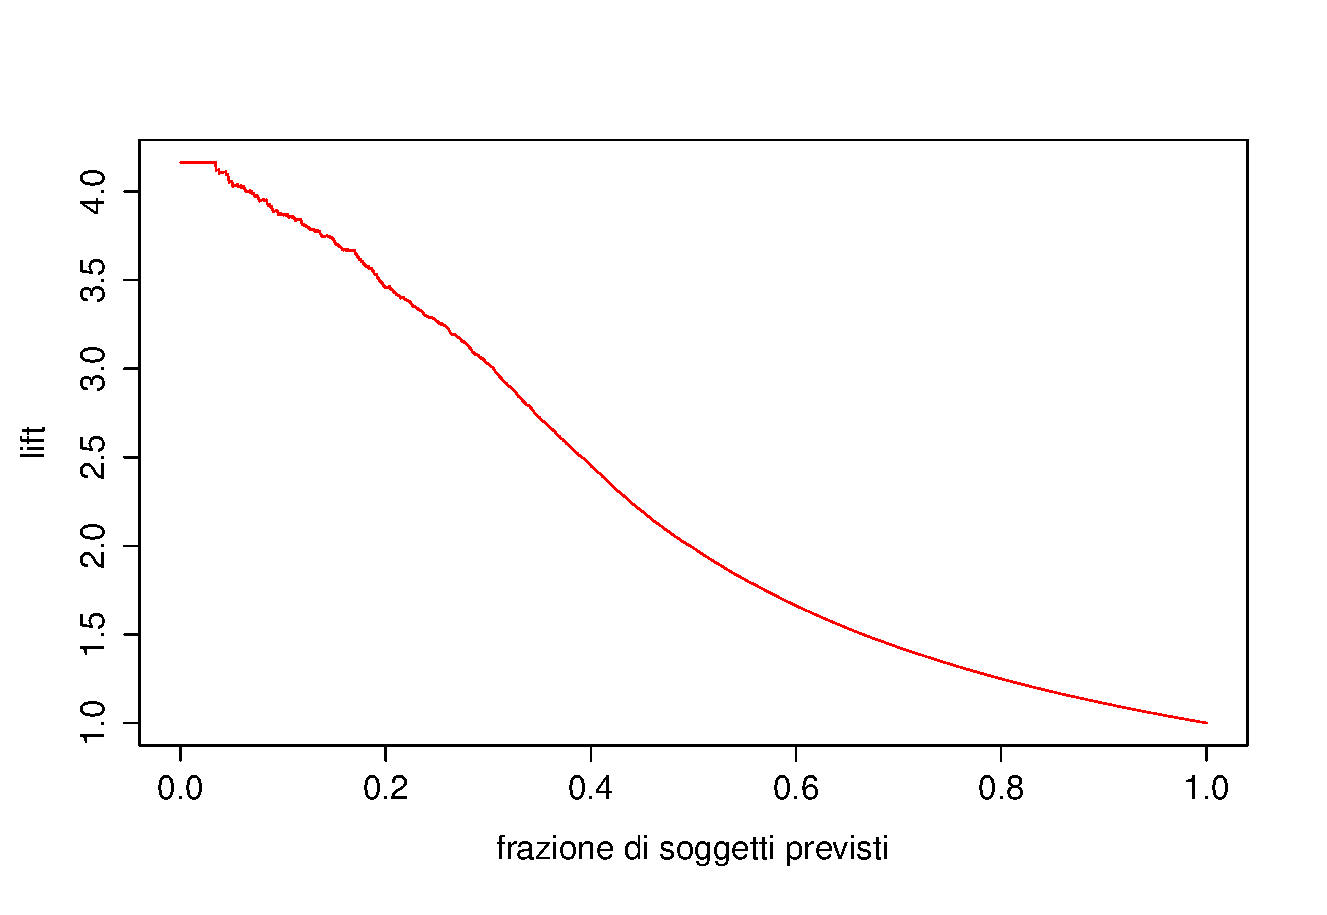
\includegraphics[width=\columnwidth]{images/class/lift-log-reg.eps}
  \end{subfigure}
  \hspace*{\fill}
  \begin{subfigure}{0.4\textwidth}
    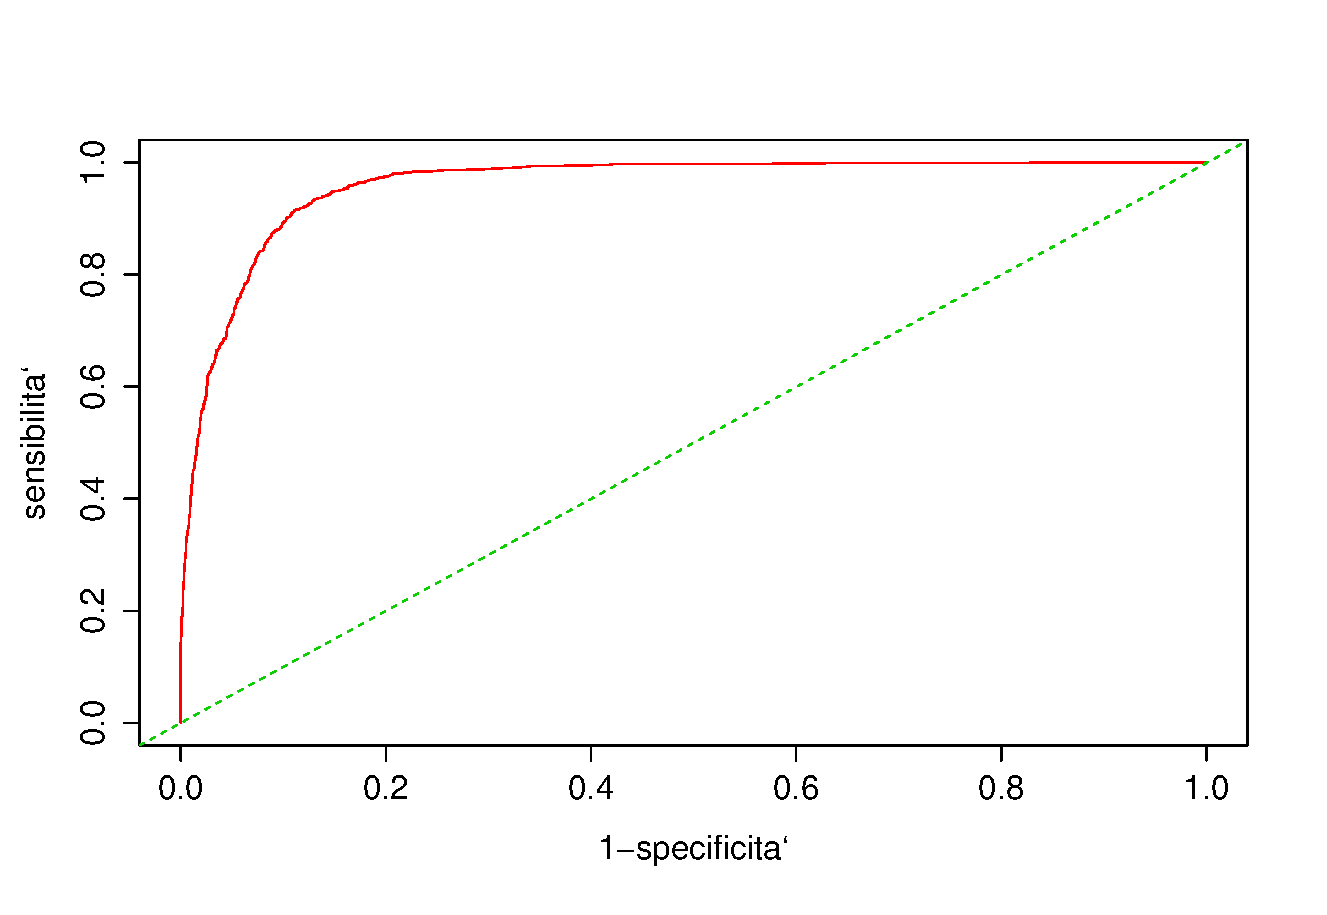
\includegraphics[width=\columnwidth]{images/class/roc-log-reg.eps}
  \end{subfigure}
  \caption{Curve per classificazione con regressione logistica}
  \label{fig:class-reg-1og}
\end{figure}

Analizzando il modello ottenuto, è possibile vedere che i fattori che più
influenzano il nostro nuovo caso di studio sono:

\begin{itemize}
\item \texttt{workingday}: come è normale aspettarsi, è la più significativa.\\
  Il numero di volte che il servizio è stato utilizzato in giorni lavorativi
  da utenti non registrati cala, poichè ci si aspetta che la maggior parte
  degli utenti casuali non risieda in Brooklyn;
\item \texttt{humidity}, al cui crescere il servizio è meno utilizzato spesso
  da utenti non registrati. \\
  Tale risultato può sembrare sensato, poichè anche nelle precedenti sezioni
  abbiamo visto che all'aumentare della temperatura il servizio veniva
  utilizzato di meno in generale nell'afosa Brooklyn;
\item \texttt{temp}: al crescere della temperatura, il servizio viene in
  generale utilizzato maggiormente e tale trend viene confermato;
\item \texttt{atemp}: come per \texttt{temp};
\item \texttt{weather}: al peggiorare delle condizioni metereologiche, il
  servizio viene utilizzato di meno da utenti non registrati. \\
  Anche questo pare sensato, poichè con condizioni metereologiche ci si
  aspetta che sia l'afflusso di turisti (i principali presupposti utenti non
  registrati) a diminuire.
\end{itemize}

%%%%%%%%%%%%%%%%%%%%%%%%%%%%%%%%%%%%%%%%%%%%%%%%%%%%%%%%%%%%%%%%%%%%%%%%%%%%%%%
%%%%%%%%%%%%%%%%%%%%%%%%%%%%%%%%%%%%%%%%%%%%%%%%%%%%%%%%%%%%%%%%%%%%%%%%%%%%%%%

\subsection{MARS}\label{sec:class-mars}

Come secondo tentativo, decidiamo di utilizzare un modello che avevamo già
utilizzato per predire la richiesta del servizio di \emph{Bike sharing} nelle
sezioni precedenti, ovvero MARS.

In questo caso cambia poco da quanto già detto in sezione \ref{sec:mars}, lo
script utilizzato è \texttt{mars-classif.R} (sezione
\ref{sec:script-mars-classif}) e anche questo usa gli stessi strumenti visti
nella sezione \ref{sec:class-log-reg} per valutare la classificazione ottenuta.

\begin{table}[H]
\begin{center}
\begin{tabular}{ | l || c | c | }
  \hline
    Previsti/Osservati & 0 & 1 \\ \hline \hline
    0 & 3907 & 384 \\ \hline
    1 & 211 & 941 \\ \hline
\end{tabular}
  \caption{Tabella di errata classificazione per MARS}
\end{center}
\end{table}

\begin{figure}[H]
  \begin{subfigure}{0.4\textwidth}
    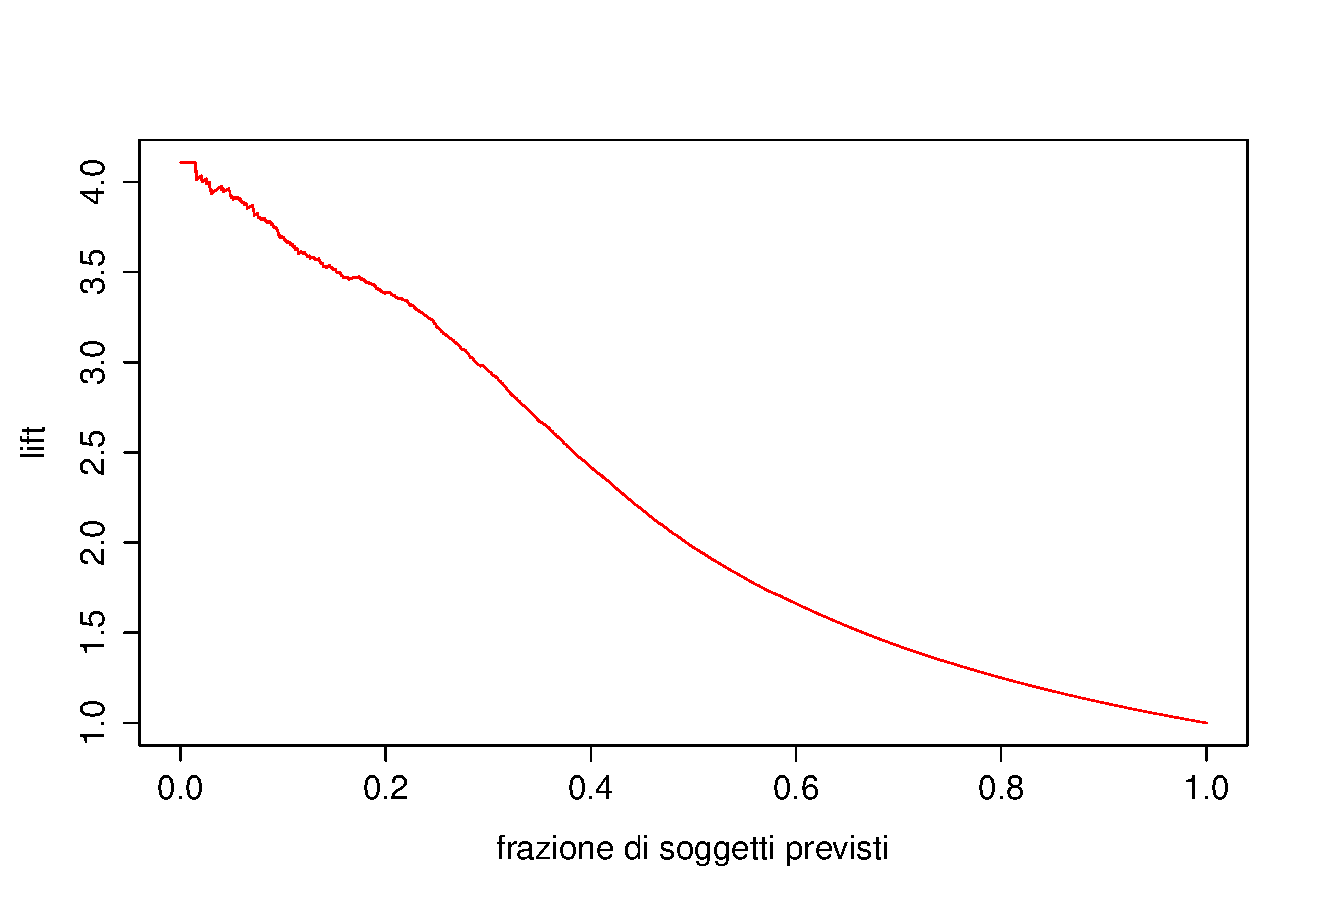
\includegraphics[width=\columnwidth]{images/class/lift-mars.eps}
  \end{subfigure}
  \hspace*{\fill}
  \begin{subfigure}{0.4\textwidth}
    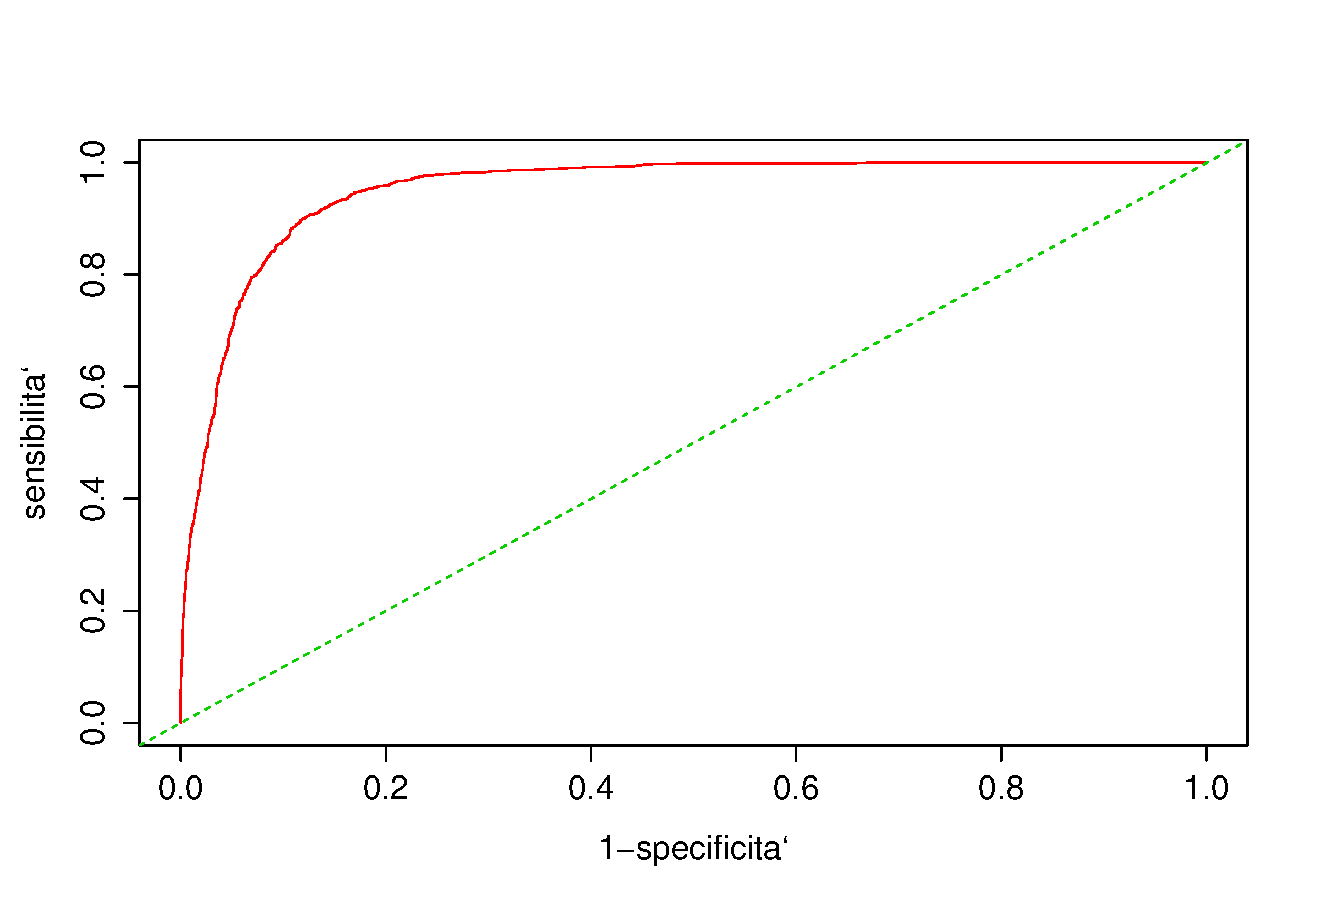
\includegraphics[width=\columnwidth]{images/class/roc-mars.eps}
  \end{subfigure}
  \caption{Curve per classificazione con MARS}
  \label{fig:class-mars}
\end{figure}

Richiedendo il grafico delle variabili più importanti per questo modello
(trovate con il comando \texttt{evimp}), \texttt{temp} e \texttt{workingday}
si confermano le più importanti per questo particolare caso di studio.

%%%%%%%%%%%%%%%%%%%%%%%%%%%%%%%%%%%%%%%%%%%%%%%%%%%%%%%%%%%%%%%%%%%%%%%%%%%%%%%
%%%%%%%%%%%%%%%%%%%%%%%%%%%%%%%%%%%%%%%%%%%%%%%%%%%%%%%%%%%%%%%%%%%%%%%%%%%%%%%

\subsection{GAM}\label{sec:class-gam}

Come terzo tentativo, anche in questo caso decidiamo di utilizzare un modello
che avevamo già utilizzato per predire la richiesta del servizio di \emph{Bike sharing} nelle sezioni precedenti, ovvero GAM.

Pure in questo caso cambia poco da quanto già detto in sezione \ref{sec:gam},
lo script utilizzato è \texttt{gam-classif.R} (sezione
\ref{sec:script-gam-classif}) e anche questo usa gli stessi strumenti visti
nella sezione \ref{sec:class-log-reg} per valutare la classificazione ottenuta.

\begin{table}[H]
\begin{center}
\begin{tabular}{ | l || c | c | }
  \hline
    Previsti/Osservati & 0 & 1 \\ \hline \hline
    0 & 3866 & 277 \\ \hline
    1 & 252 & 1048 \\ \hline
\end{tabular}
  \caption{Tabella di errata classificazione per GAM}
\end{center}
\end{table}

\begin{figure}[H]
  \begin{subfigure}{0.4\textwidth}
    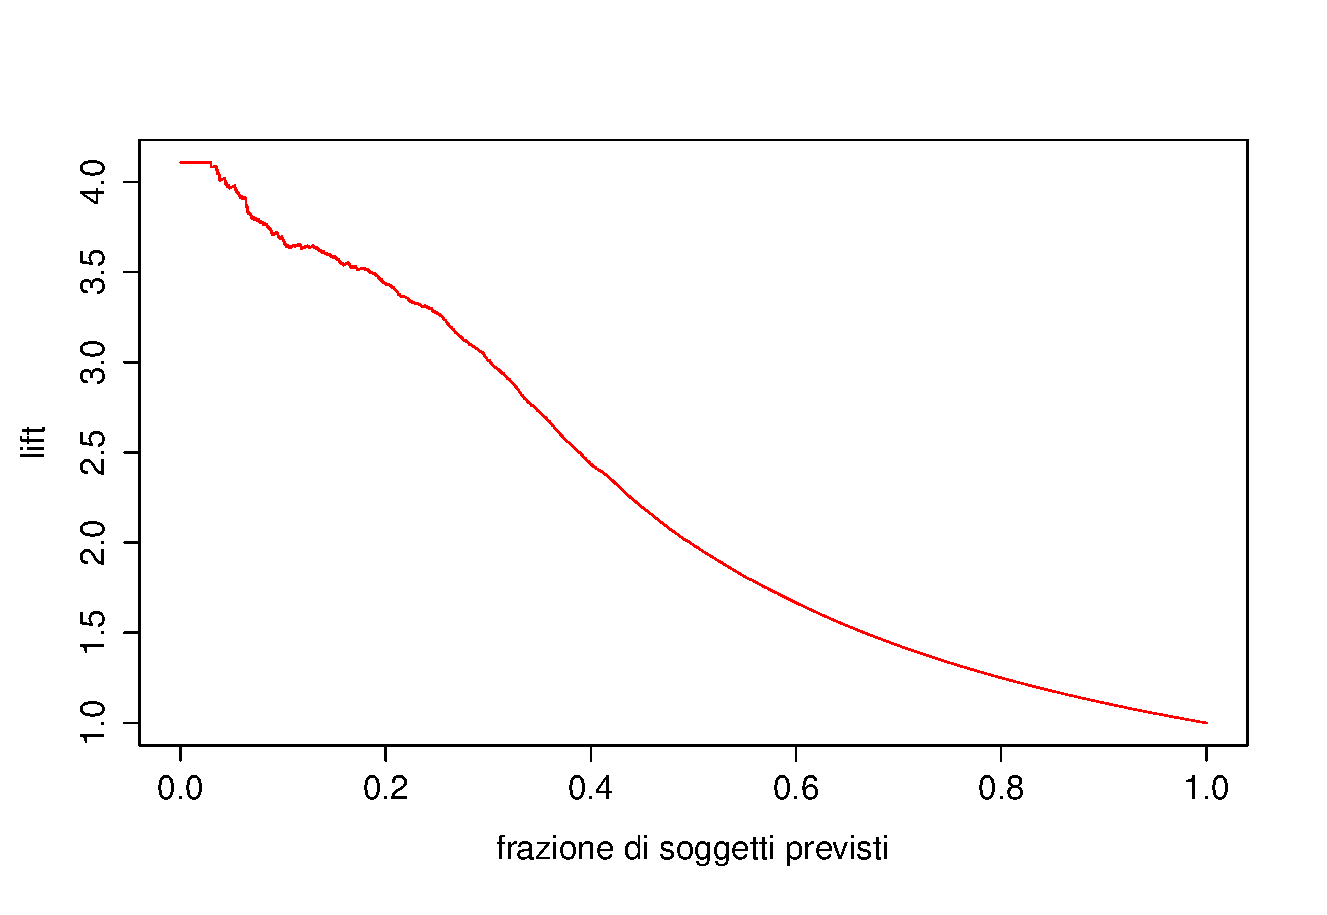
\includegraphics[width=\columnwidth]{images/class/lift-gam.eps}
  \end{subfigure}
  \hspace*{\fill}
  \begin{subfigure}{0.4\textwidth}
    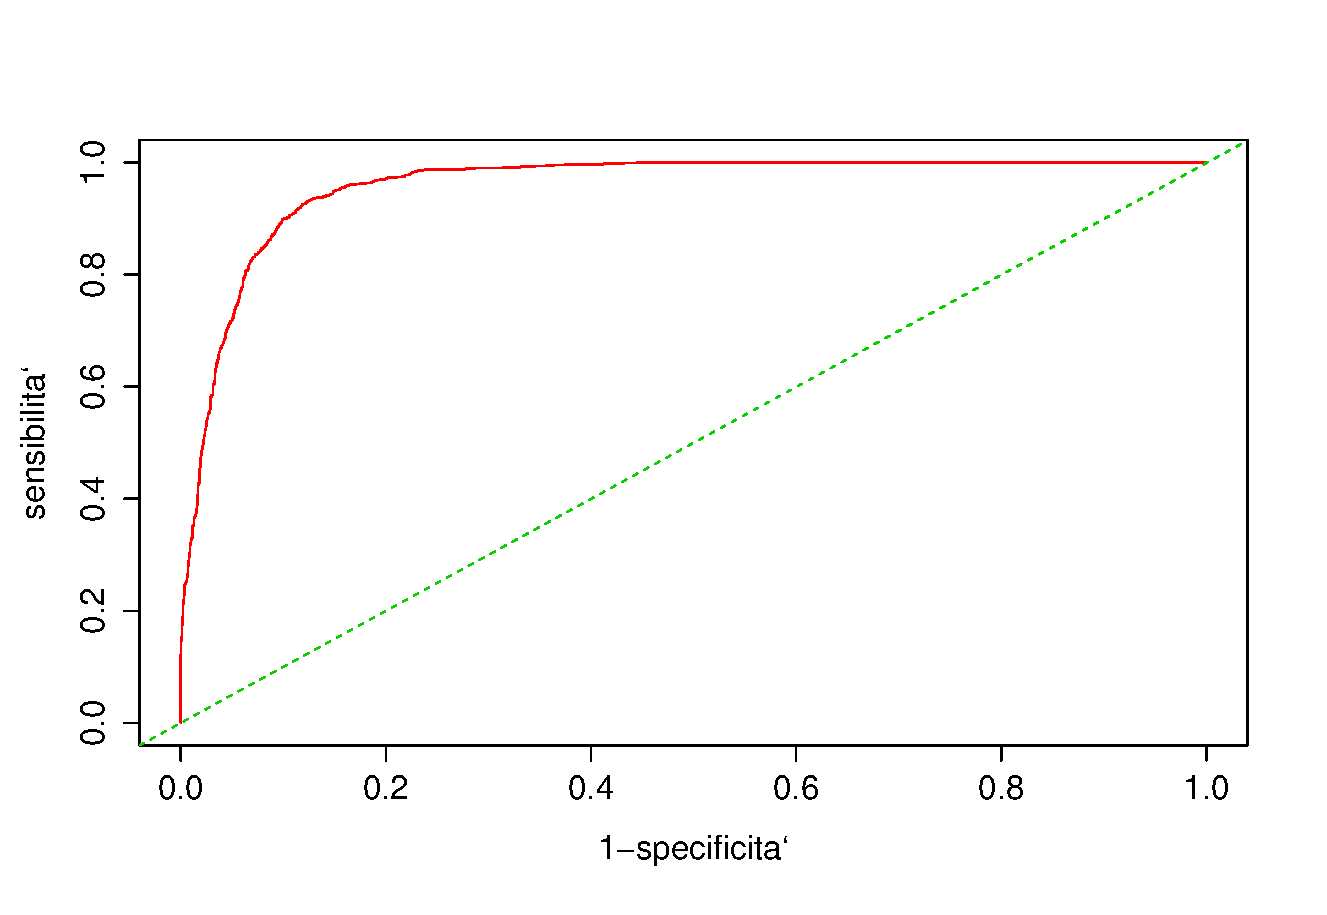
\includegraphics[width=\columnwidth]{images/class/roc-gam.eps}
  \end{subfigure}
  \caption{Curve per classificazione con GAM}
  \label{fig:class-gam}
\end{figure}

Come nella sezione \ref{sec:class-mars}, le variabili più significative sono
\texttt{temp} e \texttt{workingday}.

Anche in questo caso, dal grafico di questo modello si evince che se un giorno
è lavorativo, la richiesta del servizio da parte di utenti non registrati
cala, mentre all'aumentare della temperatura la richiesta cresce.

%%%%%%%%%%%%%%%%%%%%%%%%%%%%%%%%%%%%%%%%%%%%%%%%%%%%%%%%%%%%%%%%%%%%%%%%%%%%%%%
%%%%%%%%%%%%%%%%%%%%%%%%%%%%%%%%%%%%%%%%%%%%%%%%%%%%%%%%%%%%%%%%%%%%%%%%%%%%%%%

\subsection{Reti neurali}\label{sec:class-nnet}

Come quarto tentativo, anche in questo caso decidiamo di utilizzare un modello
che avevamo già utilizzato per predire la richiesta del servizio di \emph{Bike
sharing} nelle sezioni precedenti, ovvero una rete neurale.

Pure in questo caso cambia poco da quanto già detto in sezione
\ref{sec:neural-nets}, lo script utilizzato è \texttt{nnet-classif.R} (sezione
\ref{sec:script-nnet-classif}) e anche questo usa gli stessi strumenti visti
nella sezione \ref{sec:class-log-reg} per valutare la classificazione ottenuta.

\begin{table}[H]
\begin{center}
\begin{tabular}{ | l || c | c | }
  \hline
    Previsti/Osservati & 0 & 1 \\ \hline \hline
    0 & 3884 & 186 \\ \hline
    1 & 275 & 1098 \\ \hline
\end{tabular}
  \caption{Tabella di errata classificazione per rete neurale}
\end{center}
\end{table}

\begin{figure}[H]
  \begin{subfigure}{0.4\textwidth}
    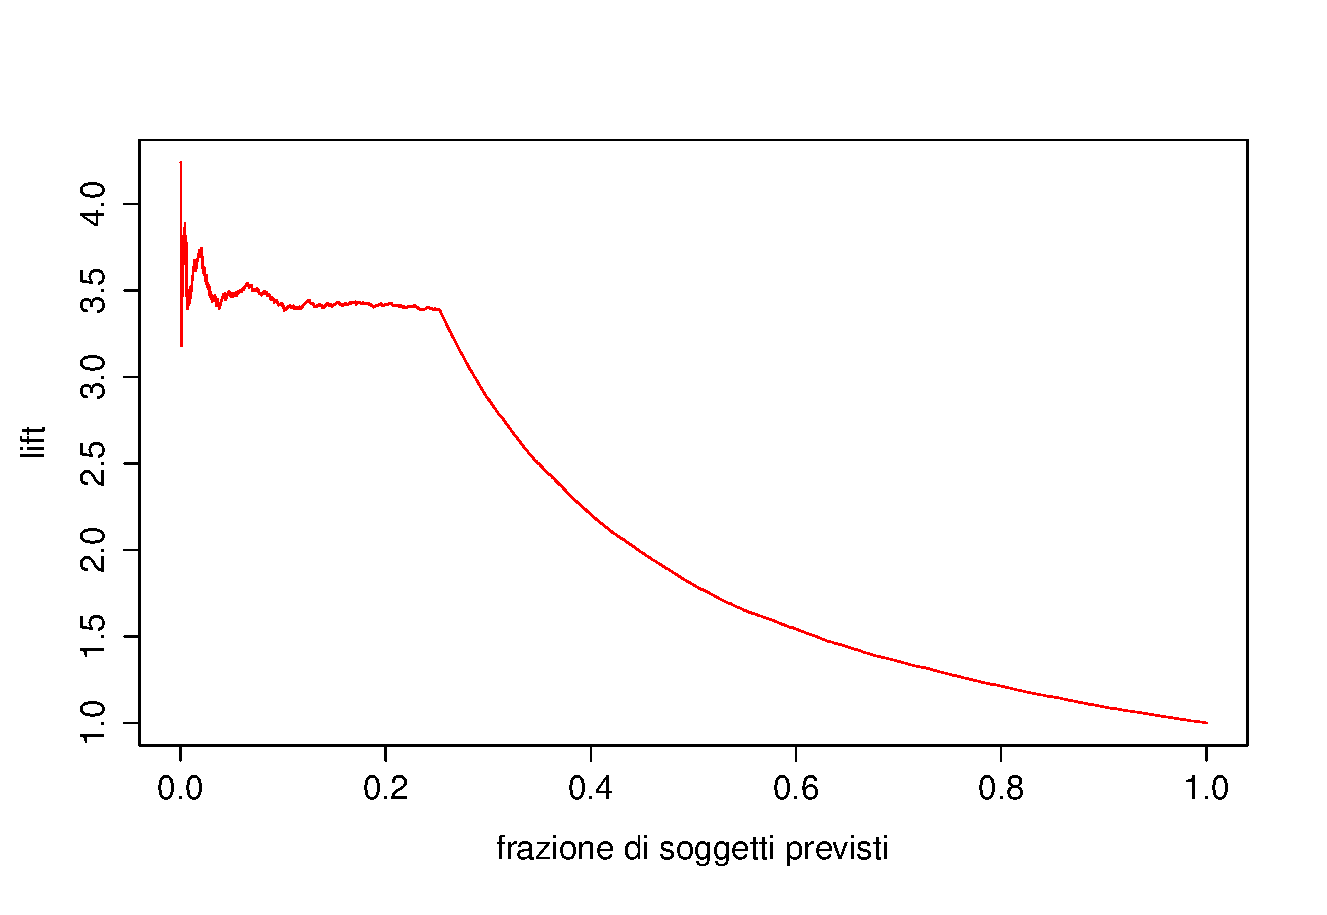
\includegraphics[width=\columnwidth]{images/class/lift-nnet.eps}
  \end{subfigure}
  \hspace*{\fill}
  \begin{subfigure}{0.4\textwidth}
    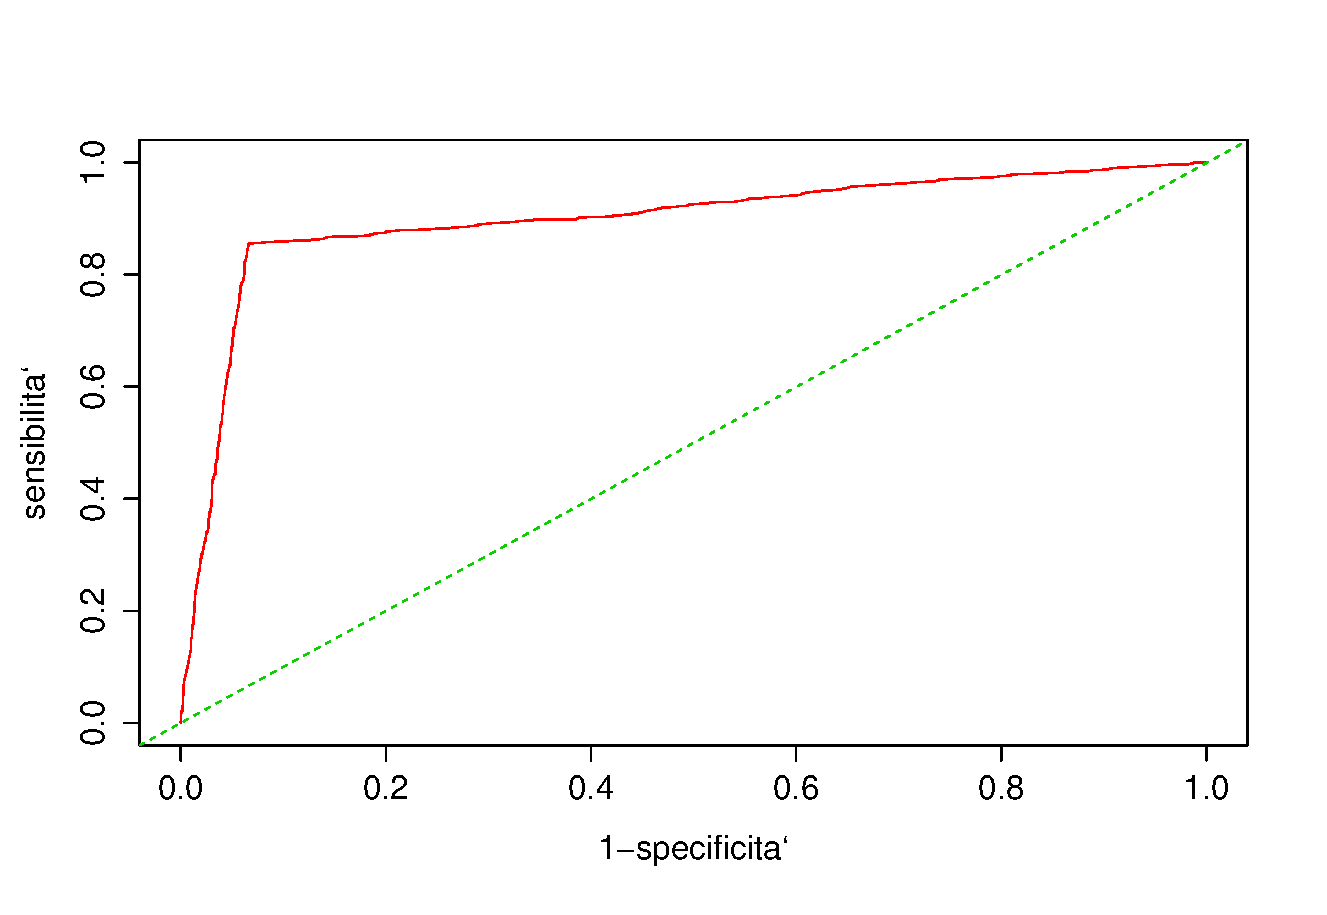
\includegraphics[width=\columnwidth]{images/class/roc-nnet.eps}
  \end{subfigure}
  \caption{Curve per classificazione con rete neurale}
  \label{fig:class-nnet}
\end{figure}

Come è possibile vedere dalla figura \ref{fig:nnet} (per questo modello non
viene riportata la rete neurale finale), le reti neurali non sono facili da
interpretare, quindi per valutarne l'efficacia utilizzeremo in seguito
solamente le curve Lift e ROC.

%%%%%%%%%%%%%%%%%%%%%%%%%%%%%%%%%%%%%%%%%%%%%%%%%%%%%%%%%%%%%%%%%%%%%%%%%%%%%%%
%%%%%%%%%%%%%%%%%%%%%%%%%%%%%%%%%%%%%%%%%%%%%%%%%%%%%%%%%%%%%%%%%%%%%%%%%%%%%%%

\subsection{Alberi di classificazione}\label{sec:class-tree}

L'ultimo modello semplice utilizzato è un albero di classificazione.

Pure in questo caso cambia poco da quanto già detto in sezione
\ref{sec:trees}, lo script utilizzato è \texttt{tree-classif.R} (sezione
\ref{sec:script-tree-classif}) e anche questo usa gli stessi strumenti visti
nella sezione \ref{sec:class-log-reg} per valutare la classificazione ottenuta.

\begin{table}[H]
\begin{center}
\begin{tabular}{ | l || c | c | }
  \hline
    Previsti/Osservati & 0 & 1 \\ \hline \hline
    0 & 3755 & 238 \\ \hline
    1 & 345 & 1105 \\ \hline
\end{tabular}
  \caption{Tabella di errata classificazione per albero di classificazione}
\end{center}
\end{table}

\begin{figure}[H]
  \begin{subfigure}{0.4\textwidth}
    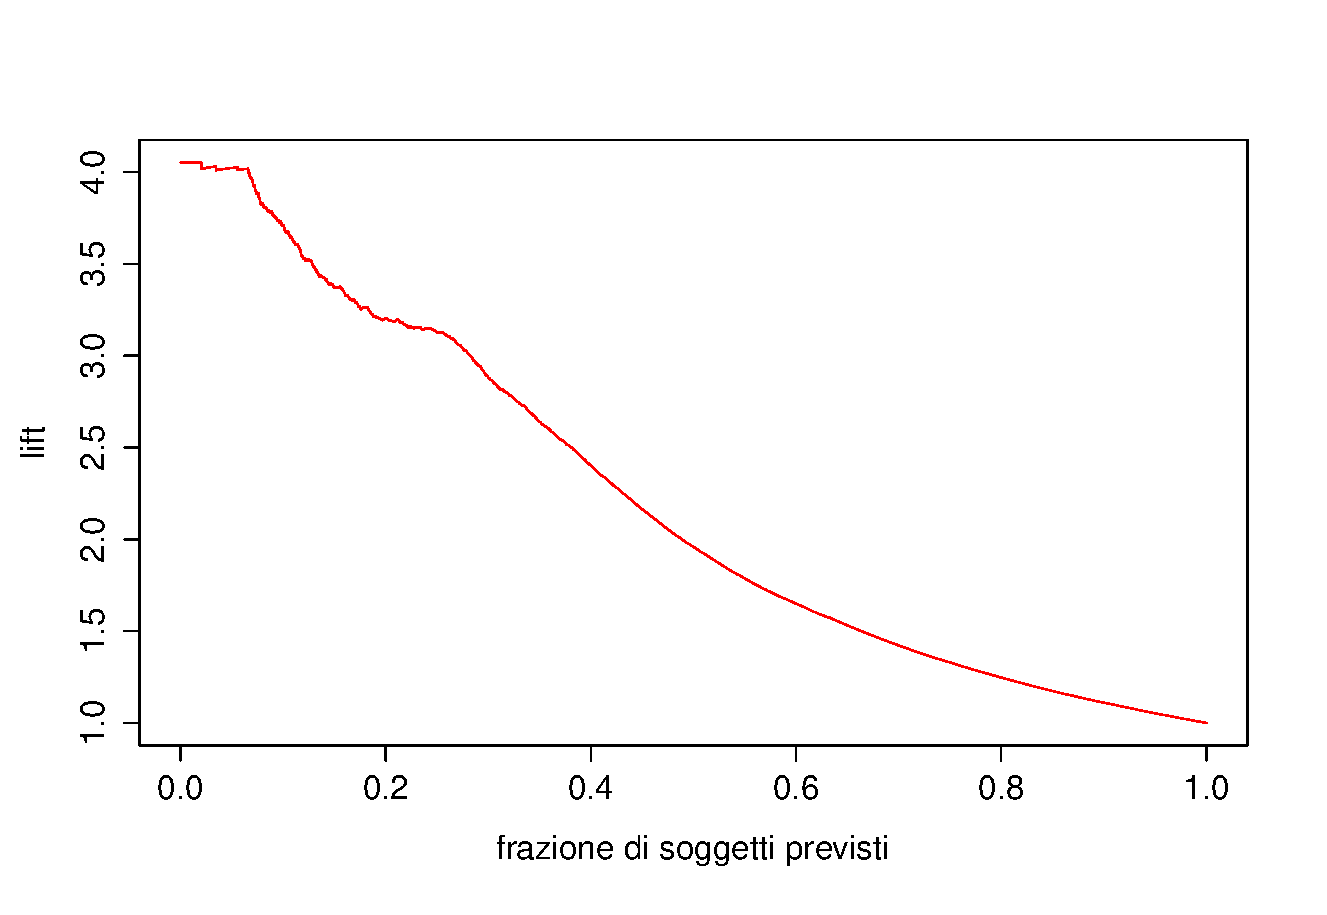
\includegraphics[width=\columnwidth]{images/class/lift-tree.eps}
  \end{subfigure}
  \hspace*{\fill}
  \begin{subfigure}{0.4\textwidth}
    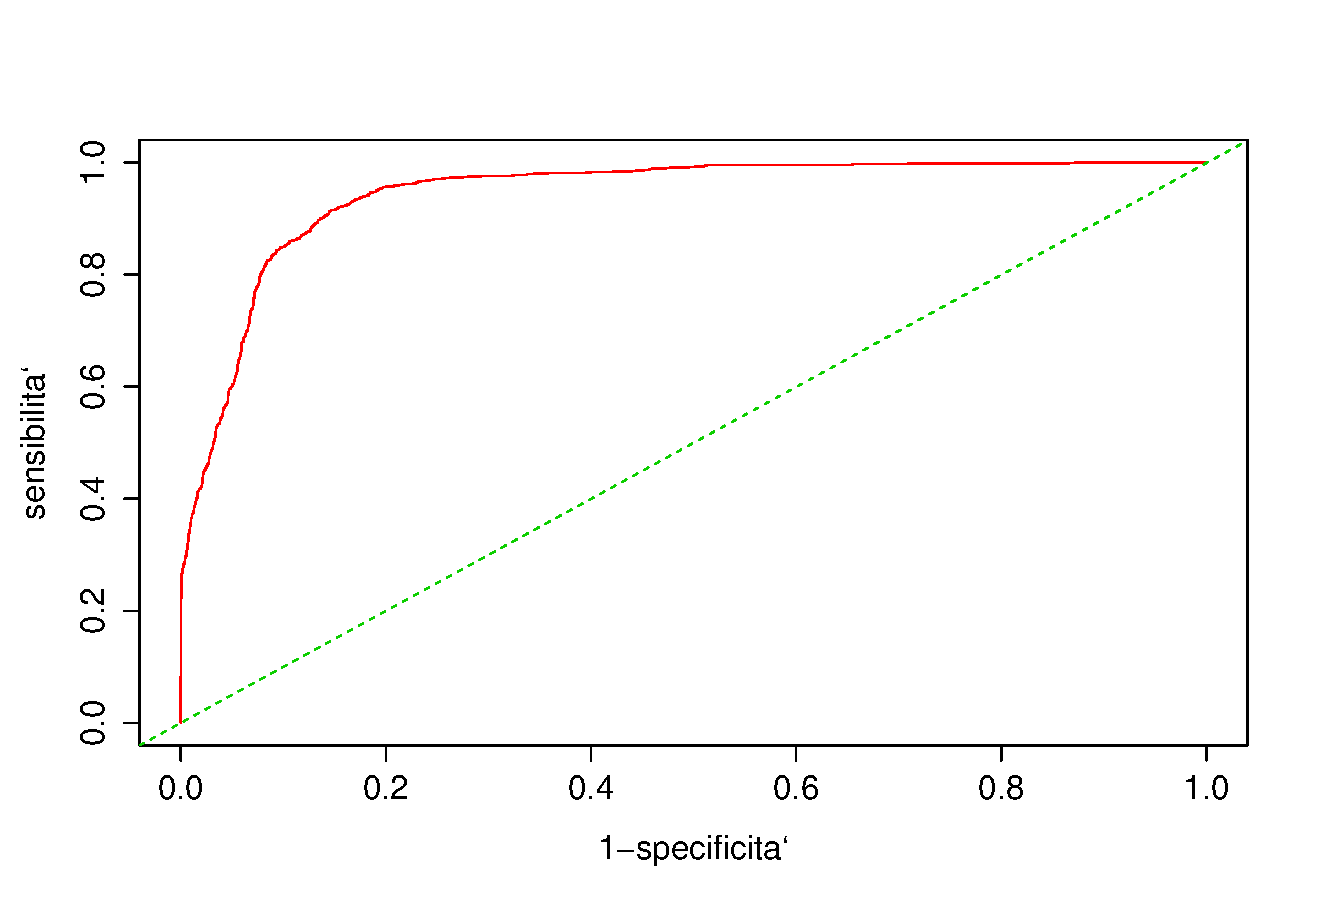
\includegraphics[width=\columnwidth]{images/class/roc-tree.eps}
  \end{subfigure}
  \caption{Curve per classificazione con albero di classificazione}
  \label{fig:class-tree}
\end{figure}

\begin{figure}[H]
  \centering
  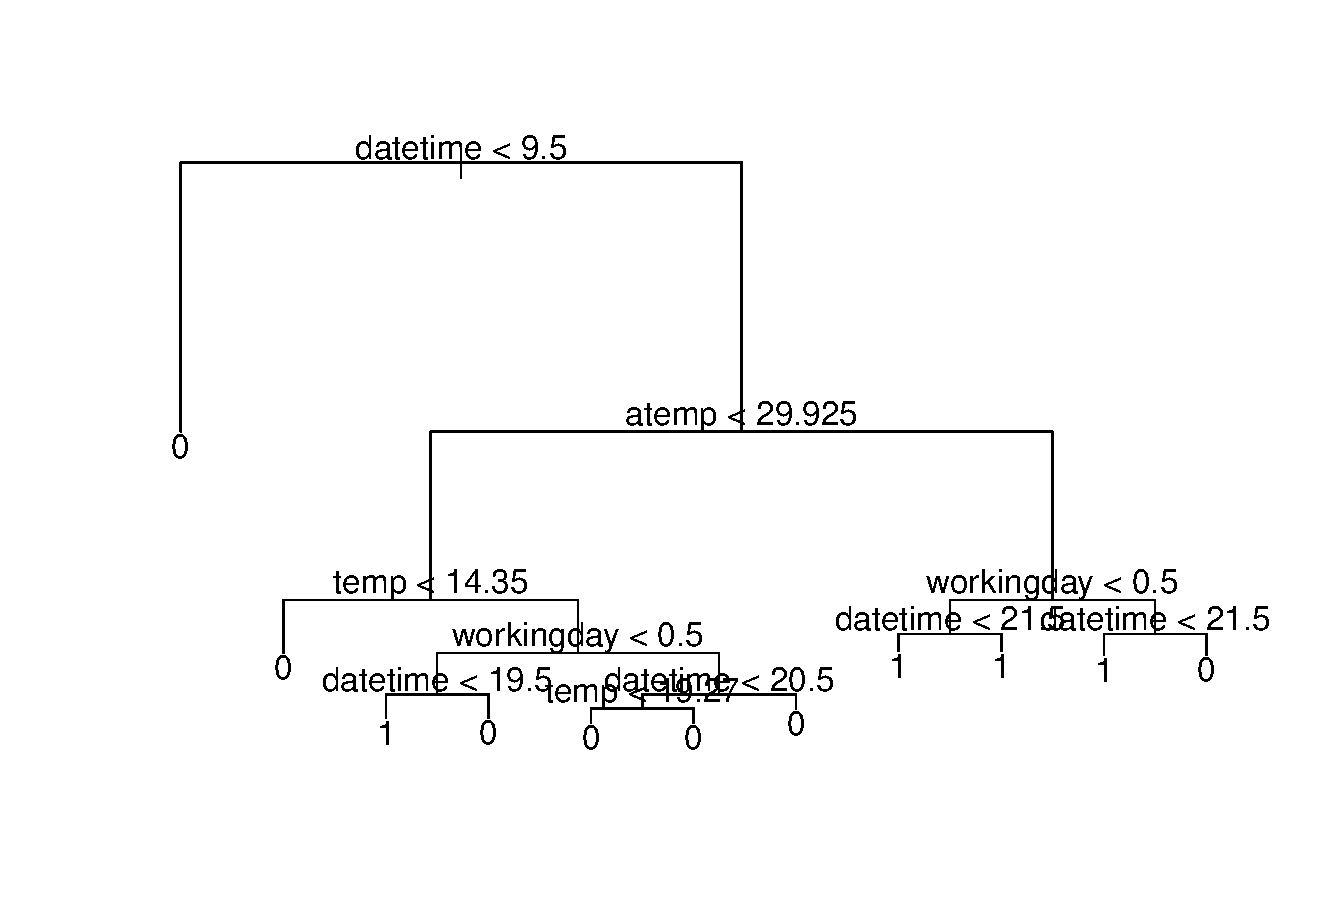
\includegraphics[width=.5\columnwidth]{images/class/final-tree.eps}
  \caption{Albero di classificazione}
  \label{fig:final-class-tree}
\end{figure}

Come in sezione \ref{sec:trees}, la dicotomia più forte per spiegare i dati è
ancora contenuta nella variabile \texttt{datetime}, decisamente determinante
per dire che il servizio di \emph{Bike sharing} è utilizzato maggiormente di
giorno (1) che di notte (0).

Guardando più attentamente le foglie dell'albero, si vedono nuovamente le
relazioni evidenziate nelle precedenti sottosezioni di questa sezione:

\begin{itemize}
\item Se fa freddo, il servizio è poco utilizzato;
\item A parità di condizioni, se il giorno non è lavorativo è più probabile
  che venga utilizzato. Analizziamo dunque i due sottoalberi che partono dalla
  condizione \emph{\texttt{atemp} $ < $ 29.925}. \\
  Nel sottoalbero sulla destra il servizio è utilizzato abbondantemente pure
  di notte se il giorno non è lavorativo. Si noti che tale ramo è figlio della
  condizione che faccia caldo, quindi molti di quei giorni potrebbero essere
  giorni estivi di vacanza. \\
  Nel sottoalbero di sinistra, il servizio è utilizzato poco se il giorno è
  lavorativo, mentre è utilizzato abbondantemente nelle ore diurne. Ci si può
  spiegare tale risultato con il fatto che se siamo nel ramo sinistro non
  siamo nelle stagioni più calde, quindi anche se la temperatura è sopra i
  14,35$^{\circ}$C le condizioni atmosferiche sono comunque maggiormente
  ostiche in confronto a quelle del sottoalbero destro.
\end{itemize}

%%%%%%%%%%%%%%%%%%%%%%%%%%%%%%%%%%%%%%%%%%%%%%%%%%%%%%%%%%%%%%%%%%%%%%%%%%%%%%%
%%%%%%%%%%%%%%%%%%%%%%%%%%%%%%%%%%%%%%%%%%%%%%%%%%%%%%%%%%%%%%%%%%%%%%%%%%%%%%%

\subsection{Bagging}\label{sec:class-bagging}

Si passa dunque a tecniche che cercano di ottenere il miglior risultato da
iterazioni in cui si tenta di applicare più volte uno stesso modello per il
nostro dataset.

Il primo tentativo, chiamato \emph{bagging}, si basa sul fatto di prelevare
casualmente parte del training set, che verrà utilizzata per trovare un CART.
Al termine del calcolo di questo, le unità verranno reinserite e potrebbero
essere estratte nuovamente dall'iterazione successiva in poi (tale metodo si
chiama \emph{bootstrap}).

Per trovare il modello finale, si assegna ad ogni classificatore la classe che
è stata prevista il maggior numero di volte per questo. Non verrà utilizzato il
\emph{bumping} per il nostro dataset poichè veramente simile al \emph{bagging},
con la differenza che non viene utilizzato un ``voto di maggioranza'' ma il
modello con minor errore viene eletto direttamente (\emph{bumps}) come modello
da utilizzare, ignorando gli altri.

In questo caso lo script utilizzato è \texttt{bagging.R} (sez.
\ref{sec:script-bagging}) e anche questo usa gli stessi strumenti visti nella
sezione \ref{sec:class-log-reg} per valutare la classificazione ottenuta.

\begin{table}[H]
\begin{center}
\begin{tabular}{ | l || c | c | }
  \hline
    Previsti/Osservati & 0 & 1 \\ \hline \hline
    0 & 3930 & 249 \\ \hline
    1 & 243 & 1021 \\ \hline
\end{tabular}
  \caption{Tabella di errata classificazione per bagging}
\end{center}
\end{table}

\begin{figure}[H]
  \begin{subfigure}{0.4\textwidth}
    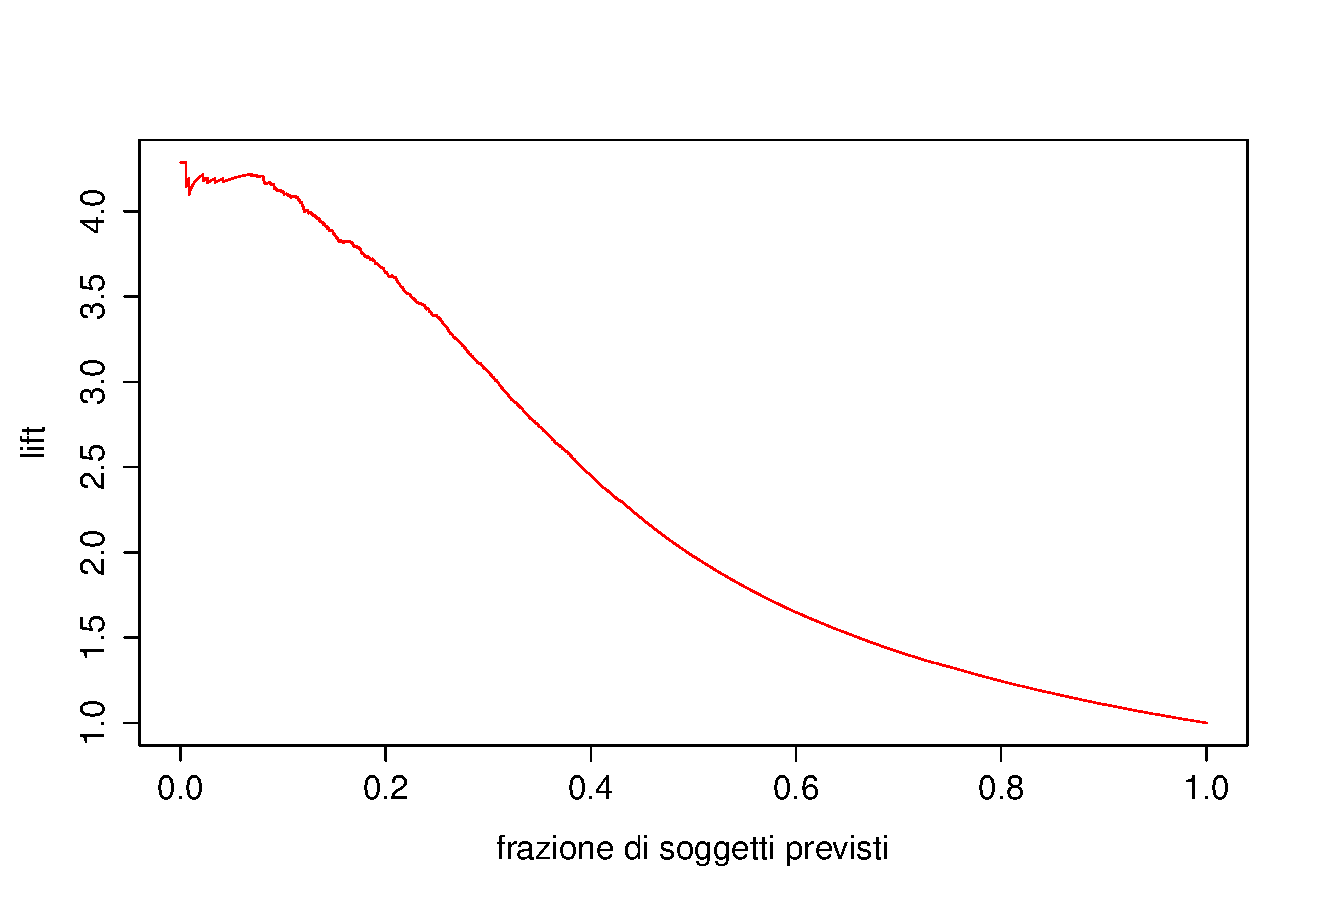
\includegraphics[width=\columnwidth]{images/class/lift-bagging.eps}
  \end{subfigure}
  \hspace*{\fill}
  \begin{subfigure}{0.4\textwidth}
    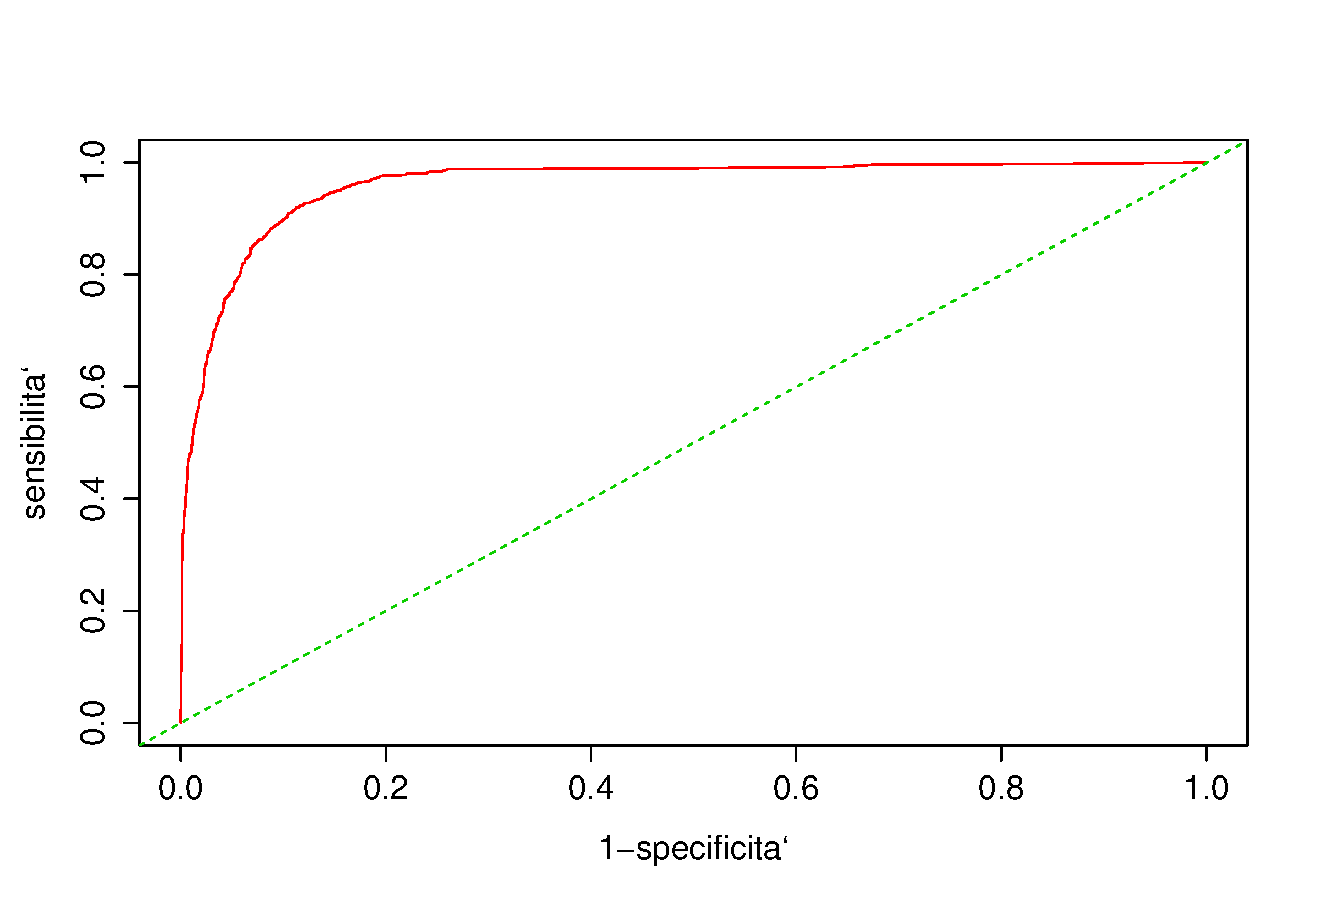
\includegraphics[width=\columnwidth]{images/class/roc-bagging.eps}
  \end{subfigure}
  \caption{Curve per classificazione con bagging}
  \label{fig:class-tree}
\end{figure}

%%%%%%%%%%%%%%%%%%%%%%%%%%%%%%%%%%%%%%%%%%%%%%%%%%%%%%%%%%%%%%%%%%%%%%%%%%%%%%%
%%%%%%%%%%%%%%%%%%%%%%%%%%%%%%%%%%%%%%%%%%%%%%%%%%%%%%%%%%%%%%%%%%%%%%%%%%%%%%%

\subsection{Boosting}\label{sec:class-boosting}

Un metodo che assomiglia al bagging ma che differisce da questo per alcune
particolarità è il boosting.

A differenza del bagging, i campioni hanno probabilità diverse di essere
estratte ad ogni iterazione. Allo stesso modo, il modello finale viene ottenuto
da una somma pesata dei modelli calcolati ad ogni iterazione.\footnote{N.B.
chiaramente è insensato far crescere l'albero fino a tutte le sue foglie,
poichè si incorrerebbe in sovradattamento}

In questo caso lo script utilizzato è \texttt{boosting.R} (sez.
\ref{sec:script-boosting}) e anche questo usa gli stessi strumenti visti nella
sezione \ref{sec:class-log-reg} per valutare la classificazione ottenuta.

\begin{table}[H]
\begin{center}
\begin{tabular}{ | l || c | c | }
  \hline
    Previsti/Osservati & 0 & 1 \\ \hline \hline
    0 & 3897 & 221 \\ \hline
    1 & 229 & 1096 \\ \hline
\end{tabular}
  \caption{Tabella di errata classificazione per boosting}
\end{center}
\end{table}

\begin{figure}[H]
  \begin{subfigure}{0.4\textwidth}
    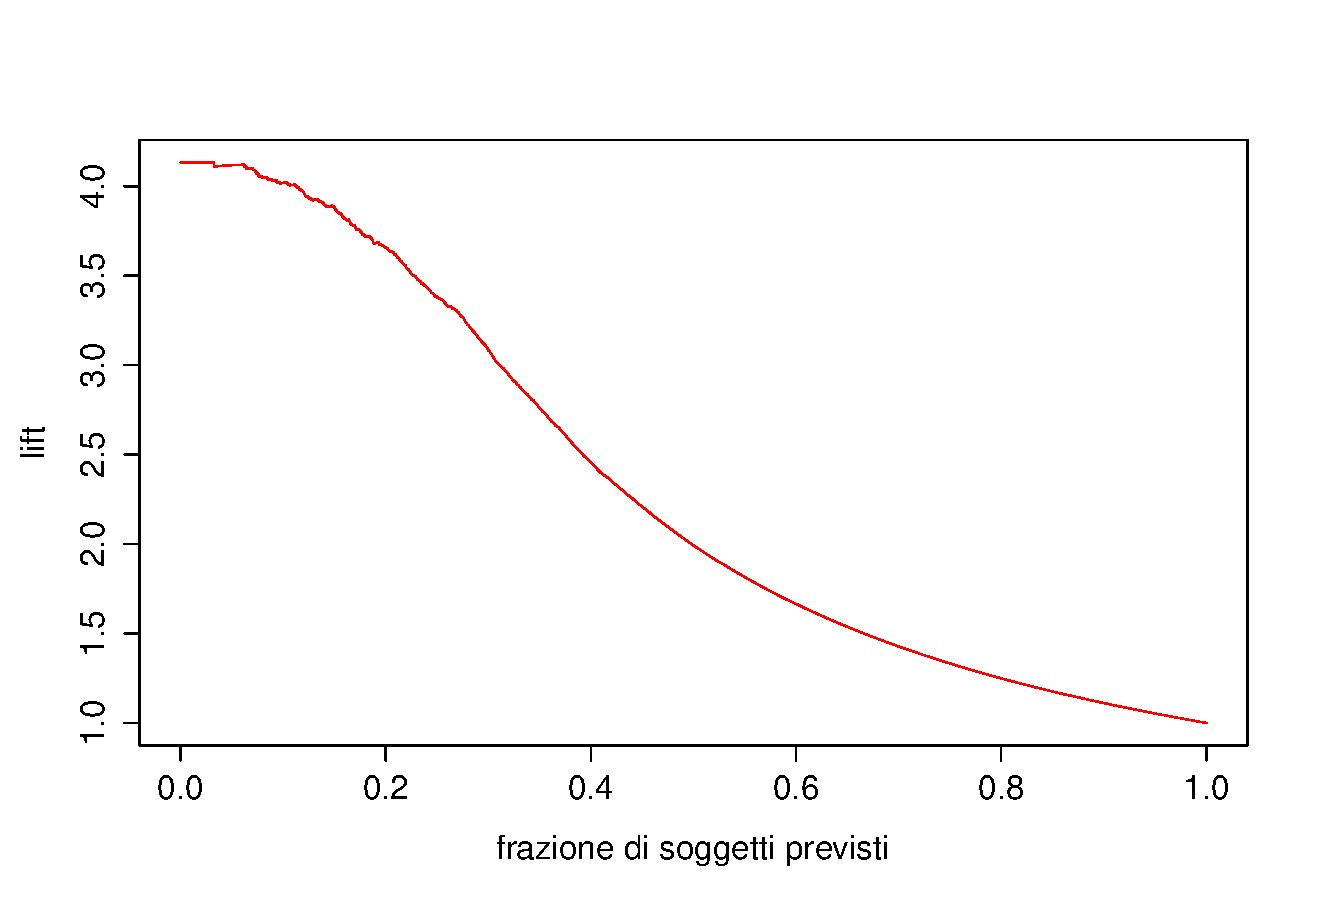
\includegraphics[width=\columnwidth]{images/class/lift-boosting.eps}
  \end{subfigure}
  \hspace*{\fill}
  \begin{subfigure}{0.4\textwidth}
    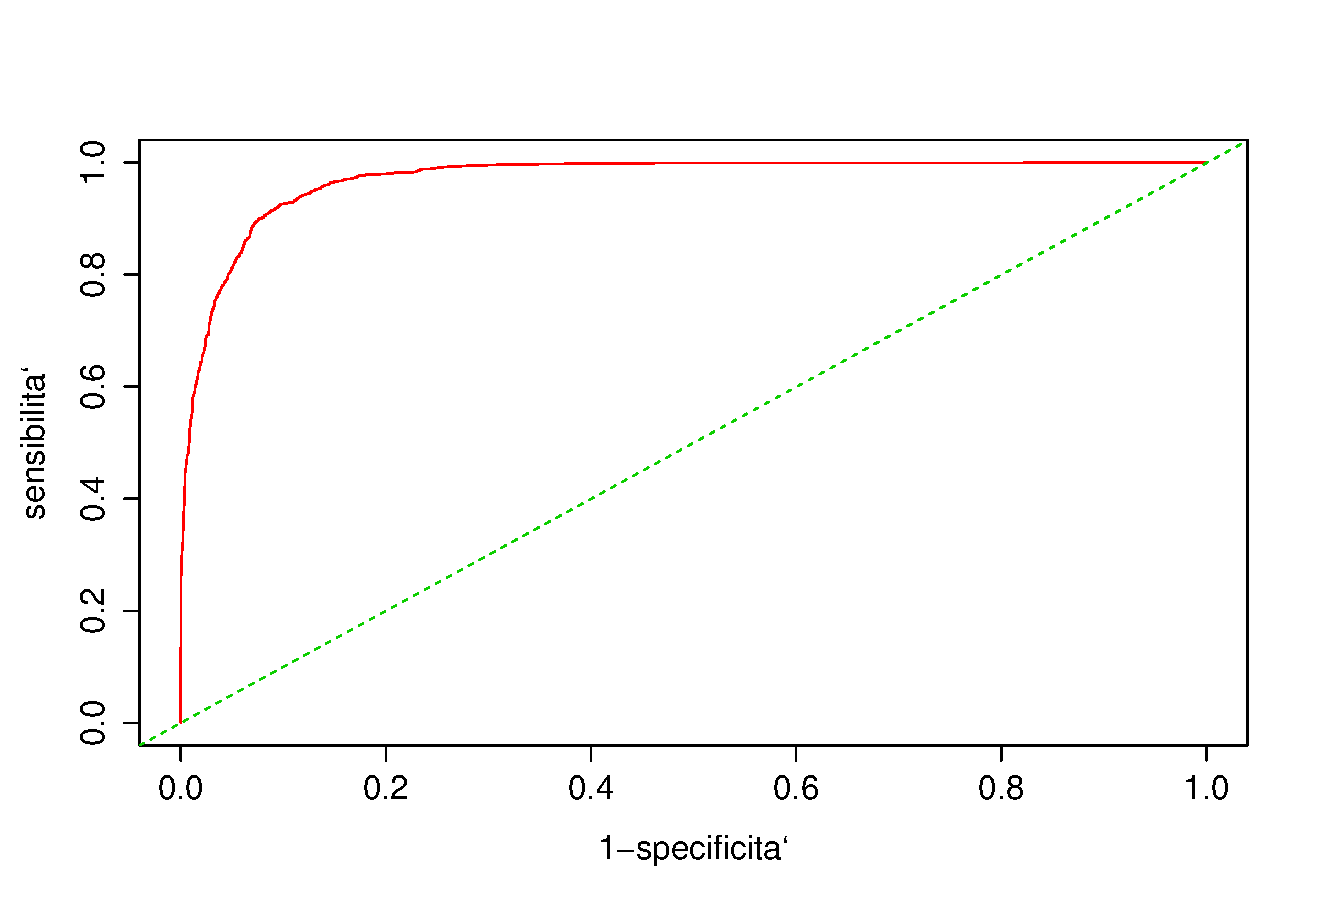
\includegraphics[width=\columnwidth]{images/class/roc-boosting.eps}
  \end{subfigure}
  \caption{Curve per classificazione con boosting}
  \label{fig:class-tree}
\end{figure}

\begin{figure}[H]
  \centering
  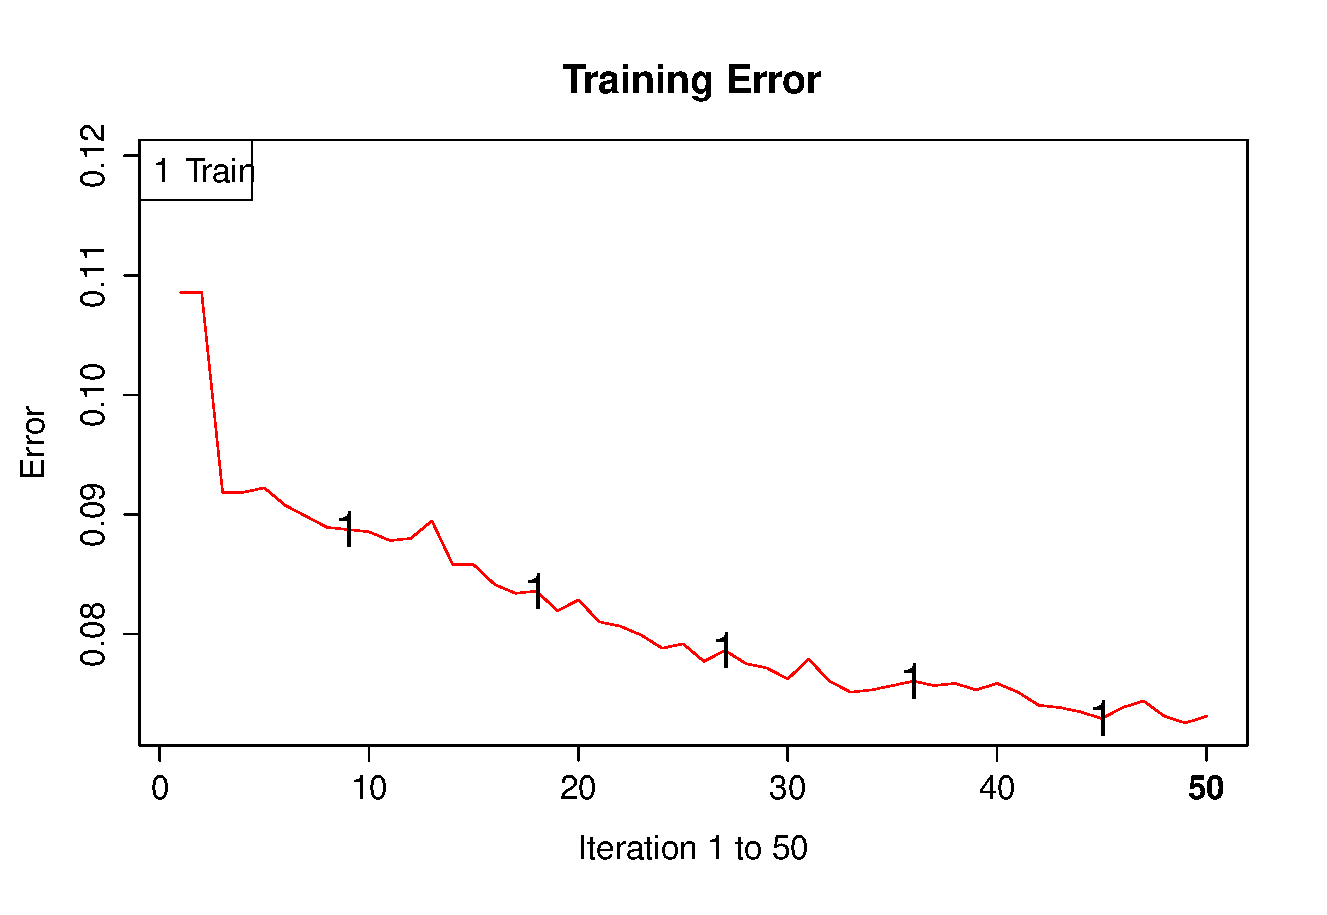
\includegraphics[width=.5\columnwidth]{images/class/boosting-plot.eps}
  \caption{Andamento dell'errore lungo le iterazioni con boosting}
  \label{fig:final-class-tree}
\end{figure}

%%%%%%%%%%%%%%%%%%%%%%%%%%%%%%%%%%%%%%%%%%%%%%%%%%%%%%%%%%%%%%%%%%%%%%%%%%%%%%%
%%%%%%%%%%%%%%%%%%%%%%%%%%%%%%%%%%%%%%%%%%%%%%%%%%%%%%%%%%%%%%%%%%%%%%%%%%%%%%%

\subsection{Random forests}\label{sec:class-forests}

Si prova ora un nuovo approccio: anzichè cambiare le unità estratte ad ogni
iterazione, si cambiano le variabili esplicative utilizzate ad ogni iterazione.

Tale metodo viene chiamato \emph{random forests}, in cui si fanno crescere
tanti alberi di regressione (ognuno con le proprie variabili) per poi
combinarne gli effetti facendo la media di questi.

In questo caso lo script utilizzato è \texttt{random-forests.R} (sez.
\ref{sec:script-rForests}) e anche questo usa gli stessi strumenti visti nella
sezione \ref{sec:class-log-reg} per valutare la classificazione ottenuta.

\begin{table}[H]
\begin{center}
\begin{tabular}{ | l || c | c | }
  \hline
    Previsti/Osservati & 0 & 1 \\ \hline \hline
    0 & 3897 & 202 \\ \hline
    1 & 252 & 1092 \\ \hline
\end{tabular}
  \caption{Tabella di errata classificazione per random forests}
\end{center}
\end{table}

\begin{figure}[H]
  \begin{subfigure}{0.4\textwidth}
    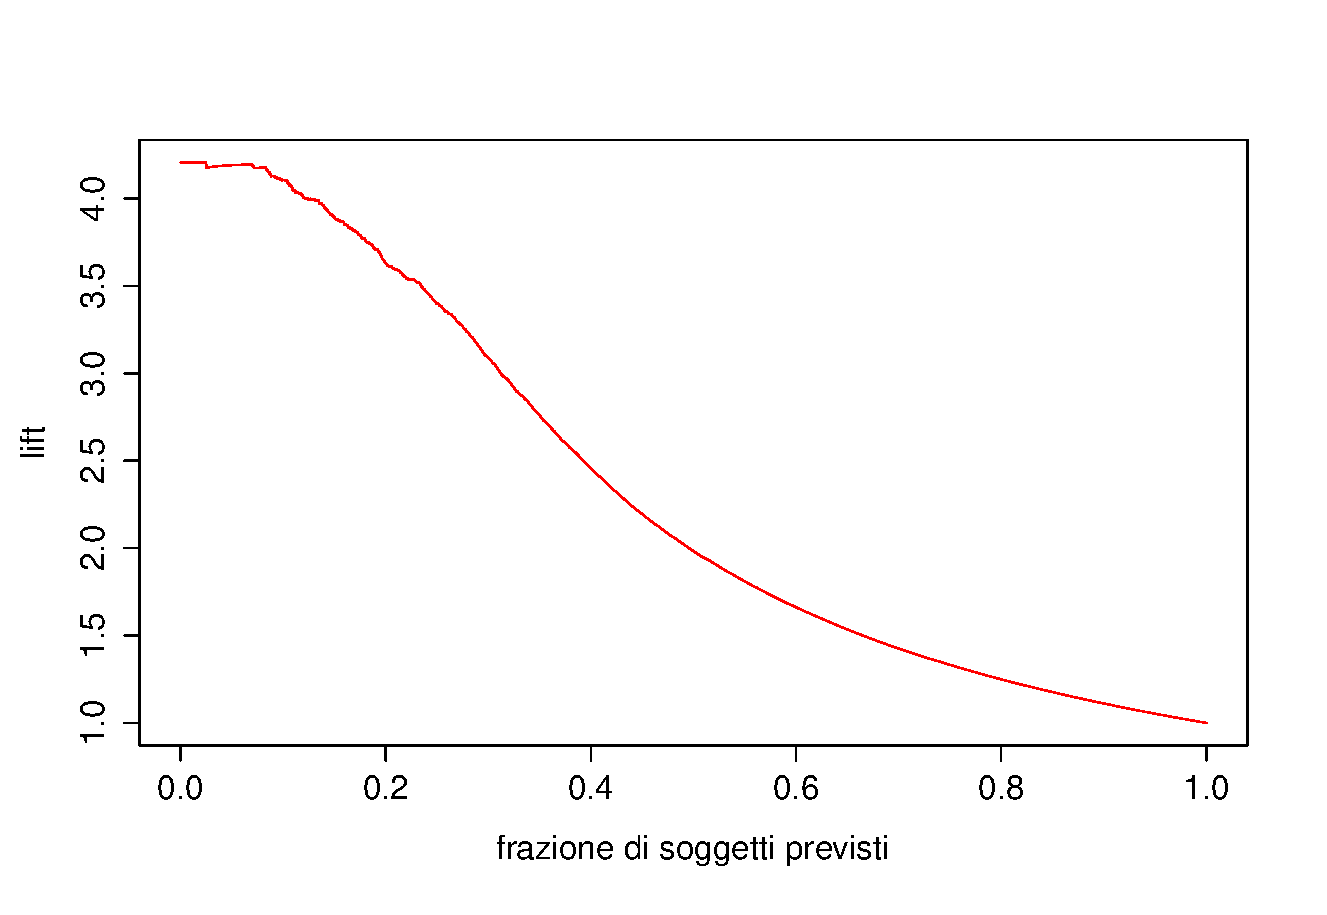
\includegraphics[width=\columnwidth]{images/class/lift-rForests.eps}
  \end{subfigure}
  \hspace*{\fill}
  \begin{subfigure}{0.4\textwidth}
    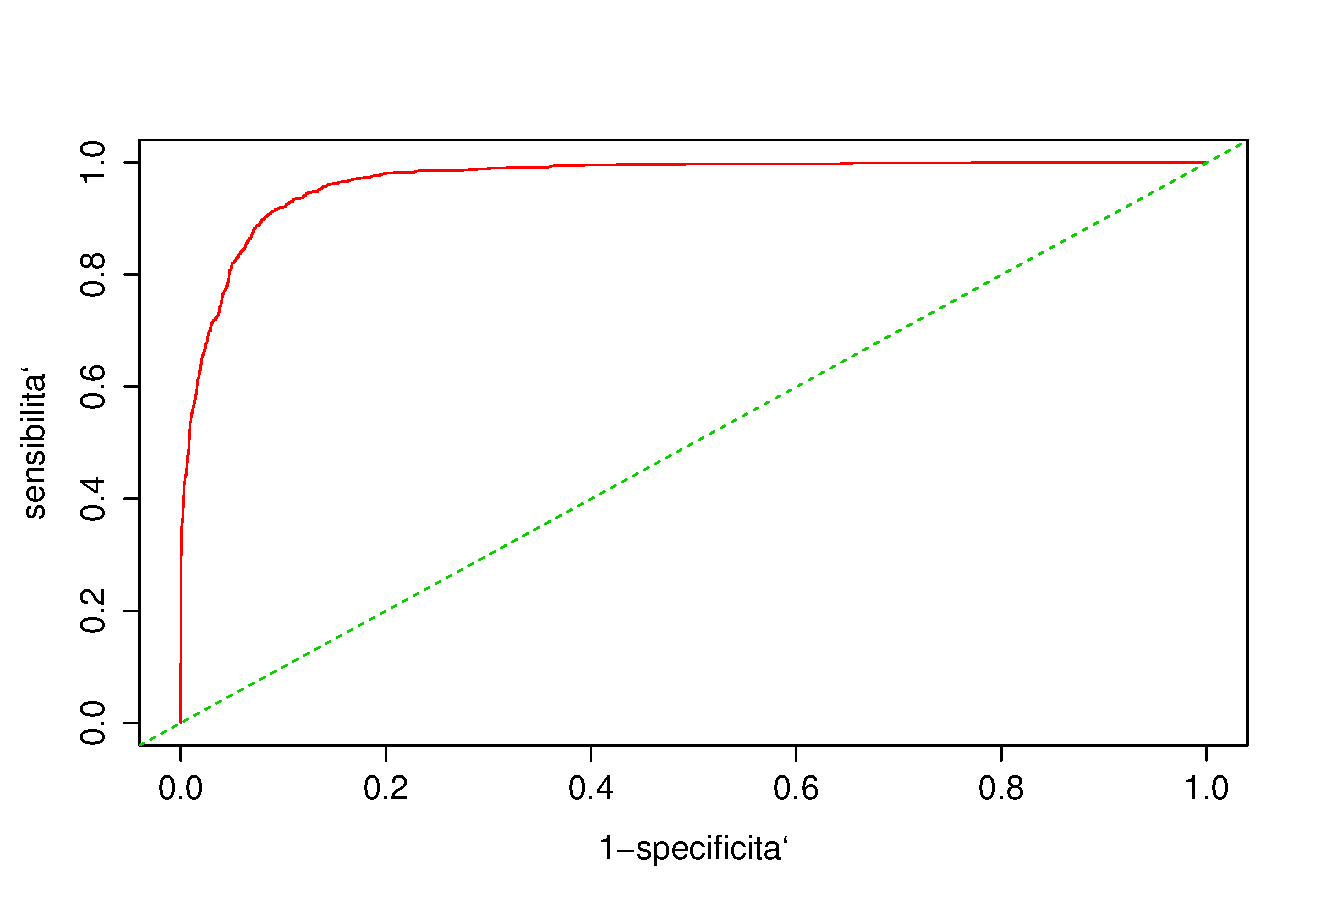
\includegraphics[width=\columnwidth]{images/class/roc-rForests.eps}
  \end{subfigure}
  \caption{Curve per classificazione con random forests}
  \label{fig:class-tree}
\end{figure}

\begin{figure}[H]
  \centering
  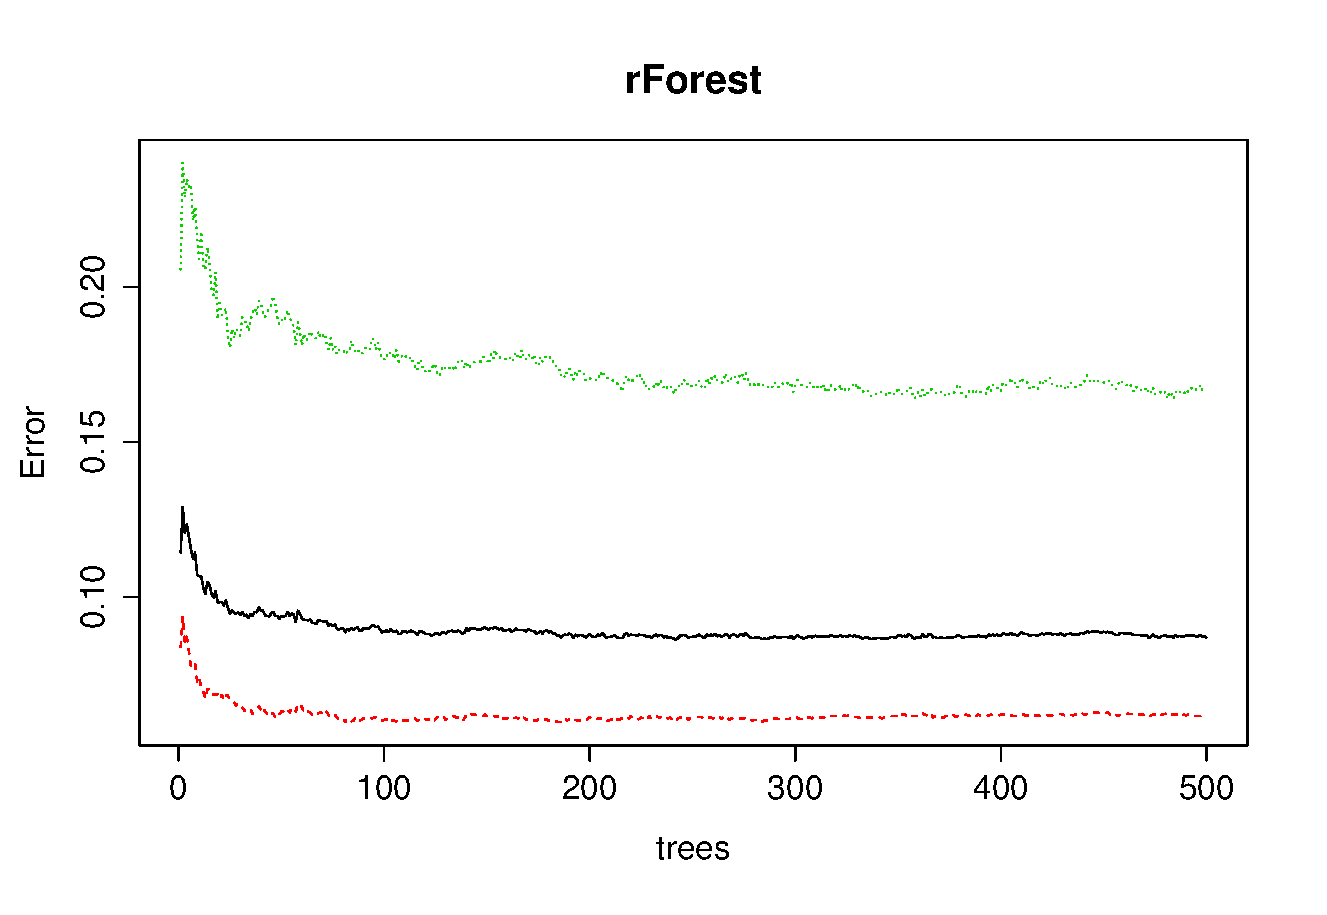
\includegraphics[width=.5\columnwidth]{images/class/rForests-plot.eps}
  \caption{Andamento dell'errore con random forests}
  \label{fig:final-class-tree}
\end{figure}

%%%%%%%%%%%%%%%%%%%%%%%%%%%%%%%%%%%%%%%%%%%%%%%%%%%%%%%%%%%%%%%%%%%%%%%%%%%%%%%
%%%%%%%%%%%%%%%%%%%%%%%%%%%%%%%%%%%%%%%%%%%%%%%%%%%%%%%%%%%%%%%%%%%%%%%%%%%%%%%

\subsection{Confronto tra modelli}\label{sec:class-comparing}

Dopo aver calcolato tutti i modelli, è opportuno compararli affinchè si possa
scegliere il migliore di questi.

Senza confrontare le curve Lift e ROC tra di loro, possiamo asserire che le
osservazioni rilevate nella sottosezione \ref{sec:class-tree} sono confermate
da tutti i modelli visti in questa sezione.

\paragraph{Lift} \mbox{} \\

Il primo confronto è tra le curve Lift, effettuato grazie agli script
\texttt{all-lifts.R} (sez. \ref{sec:script-all-lifts}) e
\texttt{plot-all-lifts.R} (\ref{sec:script-plot-all-lifts}).

\begin{figure}[H]
  \centering
  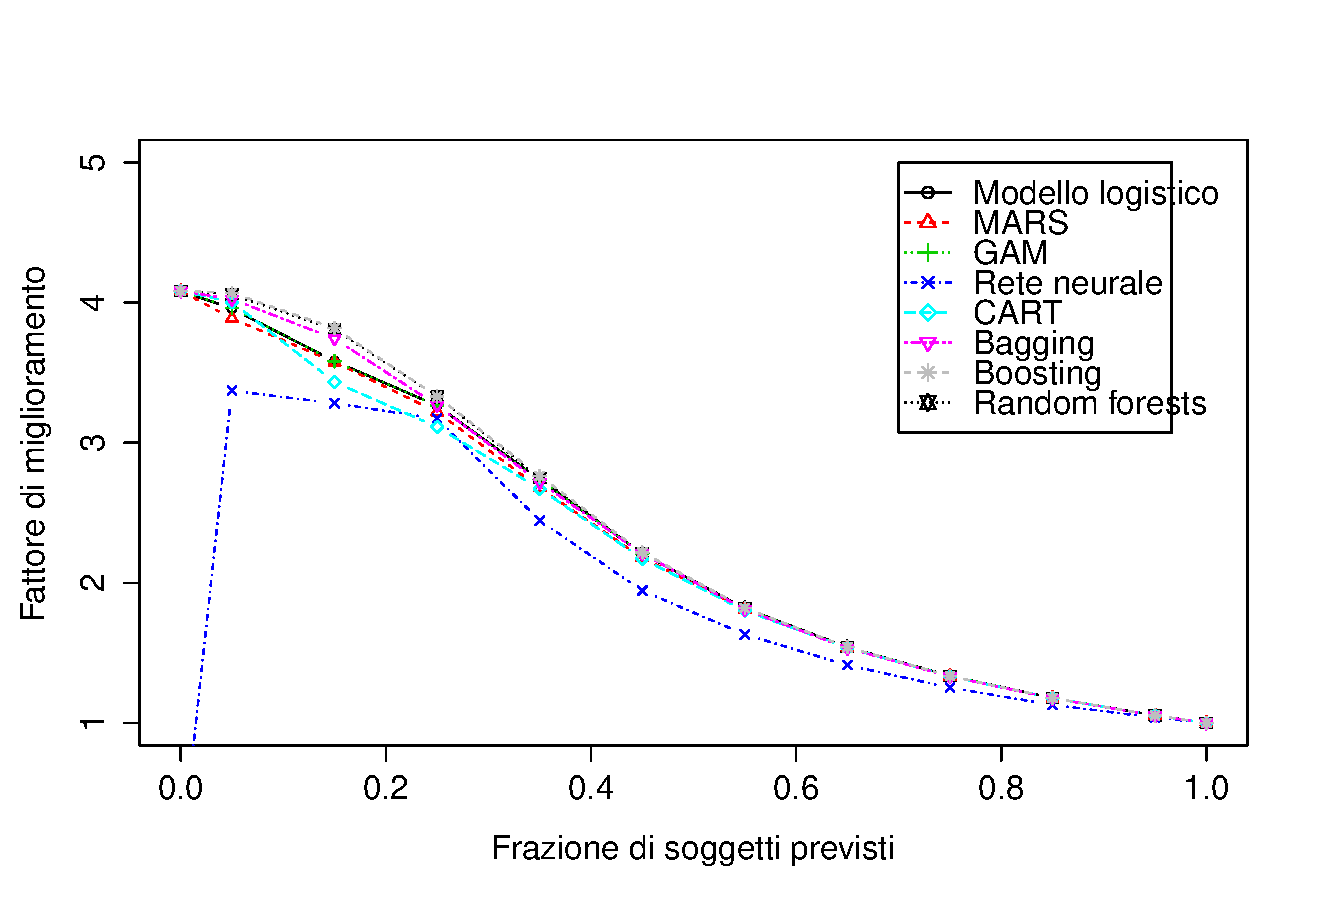
\includegraphics[width=.5\columnwidth]{images/class/all-lifts.eps}
  \caption{Confronto tra curve Lift dei modelli}
  \label{fig:all-lifts}
\end{figure}

Dalla figura è possibile vedere che tutti i modelli hanno un andamento simile
per quanto riguarda la frazione di soggetti previsti, eccezion fatta per la
rete neurale, che fornisce prestazioni sempre peggiori (e talvolta di molto).

In particolare, i tre modelli bagging, boosting e random forests riescono ad
avere un fattore di miglioramento decisamente più alto quando il campione ha
una taglia ridotta (tra il 10 e il 30\% della popolazione totale). Al di fuori
di questi intervalli, tutti i modelli hanno simile rendimento.

\paragraph{ROC} \mbox{} \\

Per quanto riguarda le curve ROC, è sufficiente lanciare lo script
\texttt{plot-all-rocs.R} (\ref{sec:script-plot-all-rocs}) dopo aver eseguito
gli script visti nel paragrafo precedente.

\begin{figure}[H]
  \centering
  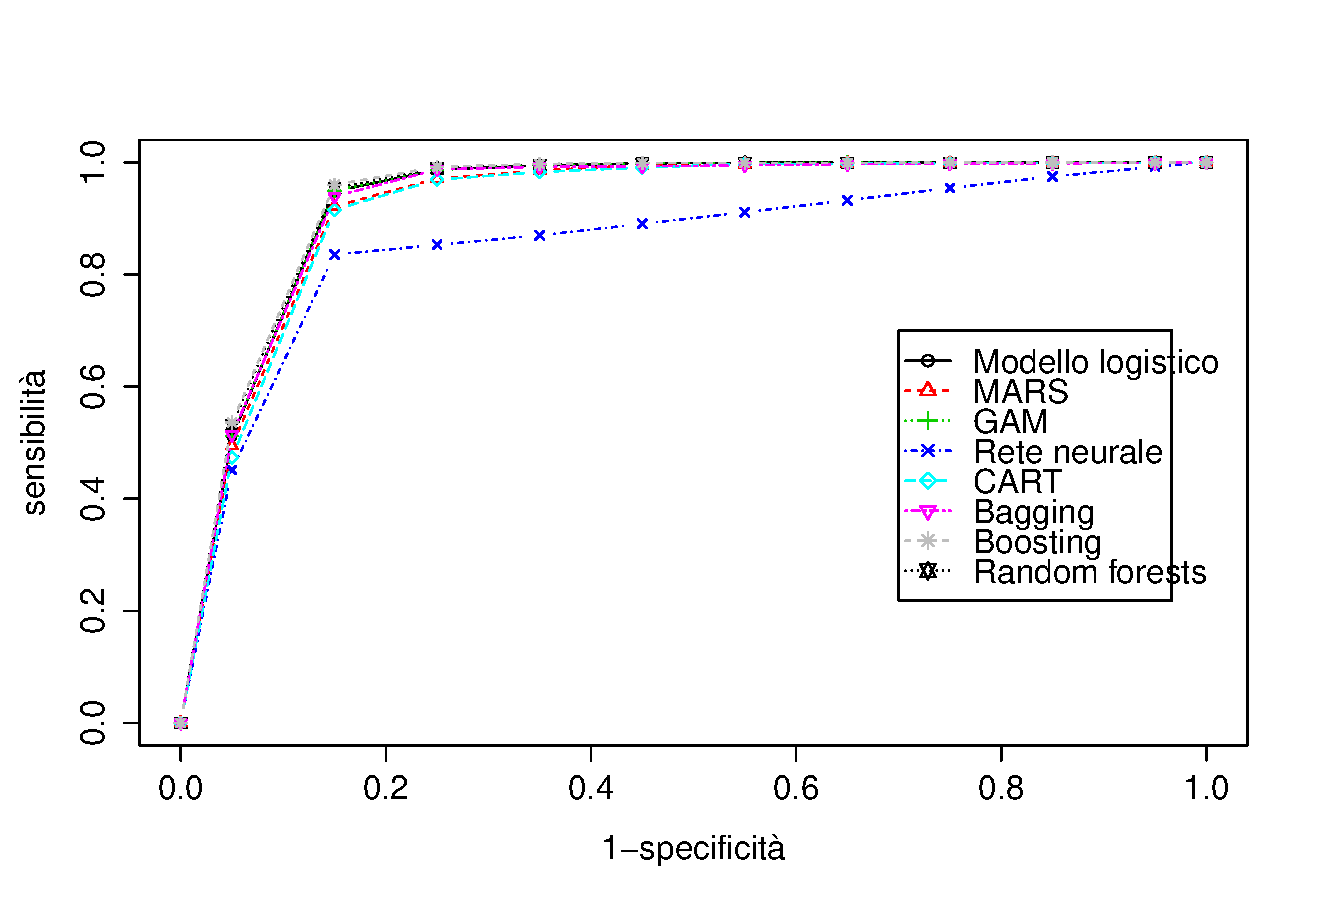
\includegraphics[width=.5\columnwidth]{images/class/all-rocs.eps}
  \caption{Confronto tra curve ROC dei modelli}
  \label{fig:all-lifts}
\end{figure}

Come è possibile vedere dalla figura sovrastante, viene confermato quanto
rilevato per le reti neurali osservando le curve Lift, il che ci sconsiglia di
utilizzarle come modello per spiegare i dati.

Per il resto dei modelli, le curve ROC sono molto vicine.

\paragraph{Considerazioni finali} \mbox{} \\

In definitiva, è possibile fare le seguenti osservazioni per il seguente caso
di studio:

\begin{itemize}
\item Per quanto riguarda questa analisi, si consiglia di non utilizzare
  \textbf{mai} le reti neurali per ottenere risultati;
\item Gli alberi di regressione sono gli strumenti più facili da interpretare
  ma forniscono prestazioni peggiori rispetto agli altri modelli;
\item MARS non è molto semplice da interpretare e fornisce risultati medi
  rispetto a tutti i modelli, quindi viene sconsigliato;
\item Dei restanti, GAM e il modello lineare logistico sono i più semplici da
  interpretare e da utilizzare ma potrebbero fornire risultati imprecisi
  quando si prelevano campioni di taglia piccola (tra il 10 e il 30\%). \\
  In ogni caso, da questi due modelli è possibile ricavare le osservazioni che
  consentono di capire in modo più chiaro quali sono i motivi alla base
  dell'utilizzo elevato di \emph{Bike sharing} da parte di utenti non
  registrati;
\item Se il campione fosse di taglia piccola, la scelta dovrebbe ricadere su
  uno dei modelli tra bagging, boosting o random forests, che hanno ottenuto i
  migliori risultati sia sulle curve Lift che ROC.
\end{itemize}

